
% Added link to preamble
\documentclass[english,12pt]{article}
\usepackage{hyperref}
\usepackage[utf8]{inputenc}
\usepackage{blindtext}
\usepackage{graphicx}
\usepackage{authblk}
%\usepackage{natbib}
\usepackage{xcolor}
\usepackage{float}
\usepackage{amsmath}
\usepackage[english]{babel}
\usepackage{graphicx} % Required for inserting images
\usepackage[paperheight=16cm,paperwidth=12cm,textwidth=8cm]{geometry}
\usepackage[flushleft]{threeparttable,booktabs}
\usepackage{tabulary,booktabs}
\usepackage{booktabs}
\usepackage{siunitx}
\usepackage{ragged2e}

\appto\TPTnoteSettings{\footnotesize}

\usepackage[
        backend=biber,
        style=authoryear-comp,
        sorting=nyt,
        style=apa
    ]{biblatex}
 \addbibresource{references.bib}


 \geometry{
 a4paper,
 total={170mm,257mm},
 left=30mm,
 right=30mm,
 top=30mm,
 bottom=30mm
 }

% Keywords command
\providecommand{\keywords}[1]
{
  \small	
  \textbf{\textit{Keywords---}} #1
}

\graphicspath{{output/}}


\addbibresource{}



\title{Trust and diversity as an outcome of associative behavior patterns}
\author{Roberto Cantillan$^{1}$, Gustavo Ahumada$^{2}$, Vicente Espinoza $^{3}$  \\
        \small $^{12}$Pontificia Universidad Católica de Chile \\
        \small $^{3}$Centre for Social Conflict and Cohesion Studies COES \\
}

\date{Junio 2023}


\begin{document}
\maketitle


\begin{abstract}
En línea con la tradición analítica de redes, buscamos profundizar en la conexión entre el comportamiento asociativo (o cívico asociativo) y resultados de capital social a nivel individual. De esta manera, nos enfocamos en las "membresías múltiples", entendidas como un mecanismo básico de constitución de un campo de relaciones interorganizacionales, y la emergencia de patrones estratificados en términos de composición y de alcance asociativo. Adicioanlmente, buscamos profundizar en la hipótesis de Putnam, la cual sugiere que las membresías asociativas se asocian positivamente con la confianza generalizada, sugiriendo que son los patrones más diversos de membresías (en efecto, aquellos que facilitan el acceso a círculos y posiciones sociales diversas) los cuales facilitan en desarrollo de capital social a nivel individual y colectivo (confianza generalizada, confianza vecinal y diversidad de contactos ocupacionales)
\end{abstract}
\hspace{10pt}

\keywords{Multiple memberships, Social capital, Trust, associative field} 

\newpage


\maketitle

\section{Introduction}

That people and communities can benefit from membership in voluntary associations is by no means a novel idea. Literature in this field has established that voluntary associations promote and enhance social relations with non-kin as well as generalized trust. Involvement in association’s activities operate as a school of civicness where individuals learn to manage their differences and process their conflicts by extending their knowledge and tolerance to people from other social circles. In addition, some researchers argue that the activation of personal ties in associations, although initially based on similar interests can help to reach distant social circles, favoring the access to scarce social resources.
\bigskip
 
To what extent positive outcomes associated accompanying voluntary associations hold in contexts of noticeable material inequality and social exclusion? In this paper we analyze the Chilean case to discuss the extent to which membership in voluntary associations contributes to social trust as well as a bridge to distant social circles. We argue that positive effects of associations regarding generalized and local trust can be discerned even in an unfavorable context. However, the quality of their connections with other voluntary organizations has a stronger effect than the type of organization.
\bigskip

Neoliberalism in Latinamerica goes hand in hand with increasing levels of social and political inequality, supported by a substantial concentration of economic resources \parencite{sassen_expulsiones_2015}. Social structure in most Latin-American countries consists of a small self-reproducing elite, a group of people below the income poverty line and roughly 70  percent of the population who is neither poor or rich. Indeed, a large proportion of the latter make do in a context of increasing uncertainty and insecurity, often engaged in informal employment \parencite{lomnitz_lo_2008, portes_free-market_2005, schneider_economic_2008}. In spite of a decreasing income poverty most of the population is vulnerable to a relapse into poverty as a consequence of individual setbacks as well as external shocks. Social policies since the 1990s in spite of their contribution to decrease acute poverty, did not revert high material inequality or offered sustainable gains to the population.
\bigskip

Neoliberal orientations somehow got ingrained in the dynamics of Chilean society fueling its long term operation. During the 1970s and 1980s, the Chilean dictatorship systematically destroyed the solidarity links in society, by sheer repression of organizations such as unions, neighbors' groups, students associations and the like. The dictatorship also dismantled the institutional support for solidarity by privatizing public services, especially pensions, education and health. On top of political repression and privatization of public services an ideology of individual achievement undermined the social fabric of Chilean society. Moreover social life itself was retracted to the private world, comprising kin and a small number of friends and acquaintances in highly homogeneous social circles (REF). Disconnection among people decreased trust in strangers hindering the conditions for collective action (Lechner ). 
\bigskip

Voluntary associations, however, continued to exist, especially in local contexts, although they are small in size and operate without coordination \parencite{espinoza_local_2013}. Voluntary associations in Chile do not match exactly the characteristics they have in the United States or Europe. Chilean groups operate at a small scale, usually associated with a neighborhood; some intend to represent the inhabitants before local authorities and others gather people with common interests (for instance, housing, recreation, sports, etc.). They usually obtain financial resources from several government funds intended to support social organization \parencite{alenda__2013}. This mechanism of public funding has affected the quality of associations because it stimulated the competition for resources among associations. Leaders of the organizations learned to compete with each other rather than cooperate, which affected the civic attributes of voluntary associations. It is debatable to what extent they meet the qualities usually associated with social capital \parencite{delamaza_sociedad_2002, espinoza_local_2013}. 
\bigskip

On top of an exclusionary model of development, individualization of social life and weak voluntary associations, political institutions have clear shortcomings in processing social and political demands, contributing to the accumulation of social discomfort. As a matter of fact the Chilean “social outburst” of October 2019, actually heralded a cycle of protest that lasted until March 2020 and was only interrupted by the sanitary crisis associated with COVID-19. Chilean protest gave way to multifarious demands pointing to a deep change in the political and economic system. We conjecture to what extent protests can be linked to many types of voluntary associations, that sheltered the many pursuits expressed in these demonstrations. (REF)
 \bigskip
 
In this paper we wonder to what extent membership in Chilean voluntary associations promotes or hinders social trust among its members. The interest of the paper has to do with the test of well-established hypotheses about the benefits of voluntary associations in a different cultural, social and political context. In the first part we contextualize and develop the theoretical argument that supports our hypotheses. We then proceed to analyze our data focusing on two levels: 1) First, we focus on the search for emerging patterns of connectivity that shape the structure of the associative field in Chile, and 2) we evaluate the effects of individual memberships in two ways of social capital: trust (local and generalized) and diversity of personal networks. Finally, we discuss our results and conclude


\subsection{Civil society in Chile and Latin America in the neoliberal phase}

The passage of time revealed the profound transformations in the relationship of the popular sectors with politics, which began with the neoliberal reforms. The neoliberal context is characterized by the replacement of the state-centric forms of the state-citizenship relationship, based on corporatism and the dominant developmentalism in Latin America until the 1970s \parencite{oxhorn_neopluralism_2004}. Instead, a market-centric pattern of state-citizenship relationship was deployed. This pattern was characterized by deploying targeted forms of incorporation and distribution of incentives, with the objective of integrating the “poor” into the market. 
\bigskip

In organizational terms, if the national popular period was characterized by the selective incorporation of popular actors in the political sphere (for example, trade unions), neoliberal reforms were the expression of the efforts of political and economic elites to exclude and weaken popular actors and their organizations, restricting their ability to influence the formulation of socioeconomic policies \parencite{collier_shaping_1991, cook_politics_2009, espinoza_local_2013, rossi_second_2015, silva_reshaping_2018}. 
\bigskip

In this scenario the traditional collective actors of the popular national matrix: unions and parties, lost their centrality \parencite{barozet_entre_2016,espinoza_local_2013,garreton_cambios_2001} and, with it, their role as intermediaries between the classes popular and the State. For the Chilean case, Espinoza (2013) suggests that the effects of neoliberal policy oriented towards the development of contests and competition for access to resources by vulnerable groups, establishes exchange relationships based on conflict instead of cooperation, which fragments local spaces and reduces solidarity between diverse groups. 
\bigskip

At the Latin American level, new popular actors with a territorial base emerged, such as indigenous peoples movements, unemployed workers, residents of marginal neighborhoods, homeless, and landless peasants \parencite{merklen_pobres_2010, rossi_second_2015, seoane_nuevas_2006, svampa_movimientos_2010}. In this context, the trade union movement was one more participant among many in the anti-neoliberal protests, and its relationship with the territorial movements varied greatly from case to case \parencite{silva_challenging_2009}. 
\bigskip

Although a heterogeneous and polycentric structure of organizations may indicate a field rich in experiences of collective action (United Nations Development Programme, 2000), integration and the capacity to mobilize resources is not assured and depends on social groups that act as bridges between these multiple experiences of collective action \parencite{baldassarri_integrative_2007, granovetter_strength_1973}. One of the characteristics that make up Chilean civil society in particular is the low capacity of popular organizations to fill structural holes. In this way, the identity heterogeneity of civil society is not accompanied by weak links between organizations, so it is plausible that the capacity for interaction, the flow of resources and solidarity is restricted. This pattern is particularly critical since the absence of stable links of cooperation and / or conflict between entities that make up a social space can also be described as a context with high levels of polarization \parencite{aref_detecting_2020}.
\bigskip

On the other hand, popular influence on public policy is less likely when channels are strongly individualized. Along these lines, the academics argued that unlike unions and other corporatist groups, the new organizations lacked party ties or privileged access to policy makers, limiting their ability to represent popular interests \parencite{collier_reorganizing_2009, silva_reshaping_2018}.
\bigskip

As the state withdrew from its basic functions, it put out to tender the space of social services. Popular demand was assumed by new non-governmental organizations (NGOs) that filled the void by providing critical services to the population  \parencite{boulding_community_2020, holzner_poverty_2007}. Many of these organizations (the vast majority of them non-profit) constituted a market that regulates the system of individual and organizational interdependencies in a focused manner, while efficiently distributing public resources to vulnerable populations. The great problem with this type of organization is that its activity is not aimed at building and / or strengthening popular coordination networks that can be constituted as links of democratic participation and governance. On the contrary, its main interest is to meet the particular and critical demands of vulnerable populations (for example, care for vulnerable minors, assistance to individuals with drug use problems, construction and basic housing), establishing dependency relationships with individuals and family nuclei. Put this way, the coordination created by this type of organization tends to be focused on individuals and to depend on permanent state surveillance \parencite{delamaza_redes_2012}.
\bigskip


\section{Theory}

Confidence in others (unknown) is one of the lowest compared to other countries in the region (Latinobarómetro). The "infrasocialized" explanations point to individuation processes marked by the ideology of individualistic entrepreneurship \parencite{araujo_desafios_2012, yopo_individualizacion_2013}. The "over-socialized" explanations point to the pressure of a system of norms that leaves little room for collective action and the development of public interest \parencite{oxhorn_neopluralism_2004}. Low civic rates and general collective participation \parencite{espinoza_capital_2009}.

\subsection{The structural bases: Collective action and trust}

The importance of memberships and patterns of interaction between voluntary associations is by no means a new idea \parencite{diani_cement_2015, sorenson_when_2014}. However, even though much of the research is based on an underlying relational theory, much of the analytical work uses aggregative descriptions to identify patterns of composition of civil society \parencite{salamon_social_1998} or ideational indicators of "cohesion" to describe the benefits of memberships \parencite{paxton_social_2002, paxton_association_2007,putnam_making_1994}. Political sociologists focus on how a cohesive civil society promotes democracy \parencite{paxton_is_1999, putnam_bowling_2000}.  Historical sociologists point to the importance of solidarity for revolutionary action \parencite{bearman_structure_1993, gould_multiple_1991}. Social epidemiologists argue that a cohesive "core" is responsible for the persistence of sexually transmitted diseases \parencite{rothenberg_personal_1996}. 
\bigskip

Structural-relational explanations point to fragmentary interaction patterns and are restricted to primary circles \parencite{castells_globalizacion_2005}. Strong polarization in the associative field and state-citizenship interaction mediated by individuals or interest groups. Collective action unfolds in highly competitive territorial contexts. Vertical fragmentation between popular and state politics (polycentric field). Low membership rate. Precarious state financing \parencite{alenda__2013}.

\subsection{Associative field, Quantity versus relations}

Voluntary associations are foci of social activity other than family, work and educational spaces \parencite{knoke_associations_1986}. In this sense, memberships have been understood as a structural characteristic that can increase the probability of acquaintances formation \parencite{mcpherson_hypernetwork_1982} and, at the aggregate level, contribute to the formation of patterns of intergroup interaction and differentiation \parencite{blau_exchange_1986}. For this reason, its ability to affect social capital distribution patterns in populations has been indicated (Benton, 2016; Diani, 1997; Feld, 1981; Glanville, 2004; Son & Lin, 2008; Tindall et al., 2012).
\bigskip

Voluntary associations are both institutions and networks embedded in broad contexts. Its deployment facilitates the emergence of an infrastructure of exchanges and interdependencies that constitute the “interstitial” field of civil society \parencite{crossley_networks_2018,diani_cement_2015,lee_when_2016}. The configuration of the field of civil society consists of a particular pattern of links (present and absent) between the set of organizational dyads \parencite{kenis_how_2002}. These patterns determine the distribution of restrictions and opportunities that affect the results of the action of the organizations and of the members of the organizations \parencite{paxton_association_2007,son_social_2008,tindall_network_2012} 
\bigskip

Along these lines, it has been suggested that memberships (conceptualized as an expression of civic commitment) contribute to improving accessibility and / or counteracting deficits in individual and collective social capital \parencite{benton_uniters_2016,small_villa_2004,son_social_2008}. On the other hand, its role as a mechanism for the integration of societies and in the functioning of democratic institutions has been recognized. For example, when the effect on the production of individual cognitive dispositions of tolerance and / or trust in other strangers is indicated \parencite{cote_social_2015,putnam_bowling_2000,tocqueville_democracy_1980} . Put like this, the benefits of memberships can be individual or collective, while contributing to the development of social capital in terms of form and content \parencite{moody_building_2009}. 
\bigskip

Voluntary associations provide an organized context for joint activities, so participation in organizations is likely to shape social networks \parencite{feld_focused_1981,mcpherson_social_1992}. In general, the analysis of social networks and associations emphasizes two aspects 1) Networks and associations are treated as contexts for socialization and the development of social cohesion. This perspective tends to emphasize mechanisms that facilitate the regulation and establishment of norms, identities and generalized trust \parencite{glanville_voluntary_2004,glanville_why_2016,paxton_association_2007,paxton_trust_2018} - public good Networks and associations are considered sources of inequality, before which individuals develop strategies to access resources and positions of influence \parencite{bekkers_social_2008} - privileged-good view. The latter is the perspective adopted by this article.
\bigskip

The logic is that greater associative contact in instances of organizational solidarity not only generates greater affection and civic virtues in general, but also has a diversifying effect on the social networks of the actors and, therefore, increases the probability of access to scarce resources \parencite{diani_social_1997,malinick_network_2013,tindall_network_2012,benton_uniters_2016}. In simple terms, it is plausible that participation in social movements fosters the development of social capital at the individual level, that is, in those who declare to be members or participate in social movements. 
\bigskip

Even though some have developed optimistic diagnoses about the development of civil society and the civic activity of popular groups in Latin America and Chile, especially after what some authors call "second incorporation" or " post-neoliberal reincorporation” \parencite{rossi_second_2015}, many of these analyzes have focused on the aggregate count of organizational experiences. For the Chilean case, \parencite{programa_de_las_naciones_unidas_para_el_desarrollo_desarrollo_2000} and the working group led by  Irarrazaval & Streeter \citeyear{irarrazaval_llona_sociedad_2017}, reported an unexpectedly rich and apparently dense reality of experiences of autonomous collective action organization. However, the perspective and, in some cases, the data used in these studies do not allow testing hypotheses associated with the structure of exchanges between types of voluntary associations or organizations. For the argument we developed, inferring a relationship structure is particularly critical. A structural approach should bring us closer to meeting that goal. We assume that any positive effect that associative life has on individuals and groups, depends on scenarios of fragmentation and segregation in the field of individual and group relationships in which the subjects are embedded. Regarding this, our aim is to analyze the emerging structure of interconnection between associative types observing the multiple memberships of individuals. According to Moody and White  \citeyear{moody_structural_2003}, this analytical focus links two levels of action: individual and organizational, and allows direct analysis of the link between local interaction and patterns of organizational intersection. The logic is that if a member belongs to two or more associations, it links those associations and thus creates a network between the associations \parencite{moody_structural_2003}. Indeed, the more independent pathways there are between groups, the more easily ideas and attitudes flow through them \parencite{moody_structural_2003}.
\bigskip

Interaction patterns between associations and not the mere number of experiences largely determine the integration of the civil society field, and the probability of exposure to diverse people (in relation to the perspective of Lester M. Salamon). The expansion of the personal networks of the members to more than one organization also creates networks between voluntary associations \parencite{moody_structural_2003, kenis_how_2002}, which may allow the transfer of resources and the trust developed within organizations towards others more or less similar. The extension of trust to distant circles involves making an assessment of the trustworthiness of individuals who do not know each other directly, which suggests that the parties are likely to focus on the predictability of each other's behavior or the average person \parencite{glanville_why_2016, paxton_association_2007, paxton_is_2015}
\bigskip

They are constituted as informal networks that depend on multiple memberships and the informal contact of members of diverse organizations. There are associations that probably overlap more with others as a result of the number of relationships that their members have with members of other associations. A proxy identified by the literature is multiple memberships \parencite{moody_structural_2003, paxton_association_2007,pena_lopez_capital_2018}. 
\bigskip

Associative field: Is made up of 1) Patterns of individual civic behavior, 2) Interaction patterns between associations and composition. 

\subsection{Voluntary associations and diversity}

An extensive body of research has focused on the role of social media in recruiting and activating memberships in voluntary associations and in the deployment of particular collective action coordination modes, such as social movements \parencite{gould_collective_1993,mcpherson_social_1992,tilly_mobilization_1978}. However, there has been less emphasis on the role of memberships in the form of personal social networks \parencite{benton_uniters_2016,tindall_network_2012}.
\bigskip

As we indicated above, it is feasible to expect that the associations most connected with their organizational environment will be foci of social activity that facilitate the intersection of diverse people and social circles, which, in turn, increases the probability of the formation of acquaintances by its members. These “known” potentials may be similar in some respects (for example, in the interest of participating in a particular type of association) but probably dissimilar in many others \parencite{erickson_social_2003}. In this way, through memberships individuals can disrupt (or reaffirm) the content and form of their personal networks. For example, increasing the range of occupations and resources achieved through the links formed in these settings, even when they are weak \parencite{benton_uniters_2016,magee_civic_2008,son_social_2008}. Given this, we suggest the following hypotheses:

\subsection{Hypothesis} 

\begin{itemize}
  \item H1: The associative behavior pattern that most connects to other associative types is positively related to generalized trust and the diversity of personal networks. 
  \item H2: The most closed associative behavior patterns (closure) are negatively related to generalized trust and the diversity of personal networks 
\end{itemize}





\section{Methodology}

Por lo general, los análisis del campo asociativo en Chile se han realizado de manera transversal, y con una perspectiva marcadamente institucional. En este contexto, nuestra apuesta es analizar la dualidad individuo/grupo (Breiger, 1979; McPherson, 1982), con una perspectiva longitudinal (4 tiempos). En específico, nos enfocamos en las membresías asociativas reportadas por los individuos y los patrones de  intersección de tipos asociativos emergentes. En términos metodológicos utilizamos el procedimiento Markov Latent Models (Bartolucci et al., 2015) considerando covariables de relevancia (ej. capital humano). Con esto podemos evaluar las probabilidades iniciales y de transición de estados latentes emergentes, generando así una imagen representativa de las tendencias de integración / desintegración del campo asociativo- voluntario chileno. Utilizamos las olas 1, 2, 3 y 4 del Estudio Social Longitudinal de Chile, ELSOC. Los resultados coinciden con lo sugerido por investigaciones anteriores toda vez que describen empíricamente el predominio de comportamientos “apáticos” y “cerrados” de la población chilena. Un patrón de comportamiento “abierto” se muestra muy minoritario, y agrupa a individuos con alto capital humano. Además, se evidencia una tendencia de segmentación por género. En general, los patrones se muestran estables en el tiempo, toda vez que hay una baja probabilidad de transición del estado “apático”, y aquellos que se muestran activos cívicamente.
\bigskip

We use the class procedure to model the assumed heterogeneity of associative behaviors at the national level. We model classes including covariates and finally we use the use of class memberships to predict the variation of general trust and diversity. The procedures have been performed with the LMest package \parencite{bartolucci_lmest_2020,bartolucci_latent_2015}, and the MplusAutomation package \parencite{hallquist_mplusautomation_2020} both designed for R environment and the Mplus v. 7.3. \parencite{muthen_mplus_2009}.

\subsection{Mixed latent class analysis with distal outcome}

They are used to explore the relationship between this variable and other auxiliary variables observed. The most stable approach is the BCH method, which uses a multiple weighted group analysis, where the groups correspond to the latent classes \parencite{bakk_relating_2014}.
\bigskip

The BCH method uses weights wij that reflect the measurement error of the latent class variable. In estimating the auxiliary model, its observation in class / group j is assigned a weight of wij and the auxiliary model is estimated as a multiple-group model using these weights. 

\section{Results}

\subsection{Latent class analysis}

% latex table generated in R 4.1.2 by xtable 1.8-4 package
% Thu Jun  1 17:43:38 2023
\begin{table}[H]
\centering
\begin{threeparttable}
\caption{\label{demo-table} Fit statistics of class models}
\begin{tabular}{rrrrrr}
  \hline
 & states & lk & np & aic & bic \\ 
  \hline
1 & 1.00 & -14394.87 & 8.00 & 28805.74 & 28848.76 \\ 
  2 & 2.00 & -13586.64 & 46.00 & 27265.28 & 27512.66 \\ 
  3 & 3.00 & -12965.46 & 104.00 & 26138.91 & 26698.20 \\ 
  4 & 4.00 & -12734.50 & 102.00 & 25833.01 & 26811.76 \\ 
  5 & 5.00 & -12523.17 & 200.00 & 25606.33 & 27112.11 \\ 
   \hline
\end{tabular}
\begin{tablenotes}
    \item[1] According to the BIC relative adjustment statistic, it is the model of 3 classes or latent states.
  \end{tablenotes}
\end{threeparttable}
\end{table}


\begin{figure}[htp]
    \centering
    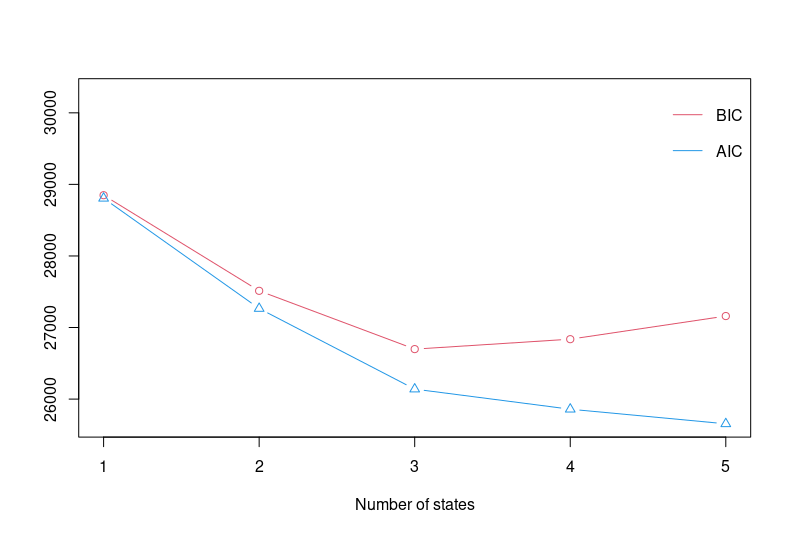
\includegraphics[width=15cm]{output/plot_fit.png}
    \caption{Fit statistics of class models 2}
    \label{fig:galaxy}
\end{figure}


\begin{figure}[htp]
    \centering
    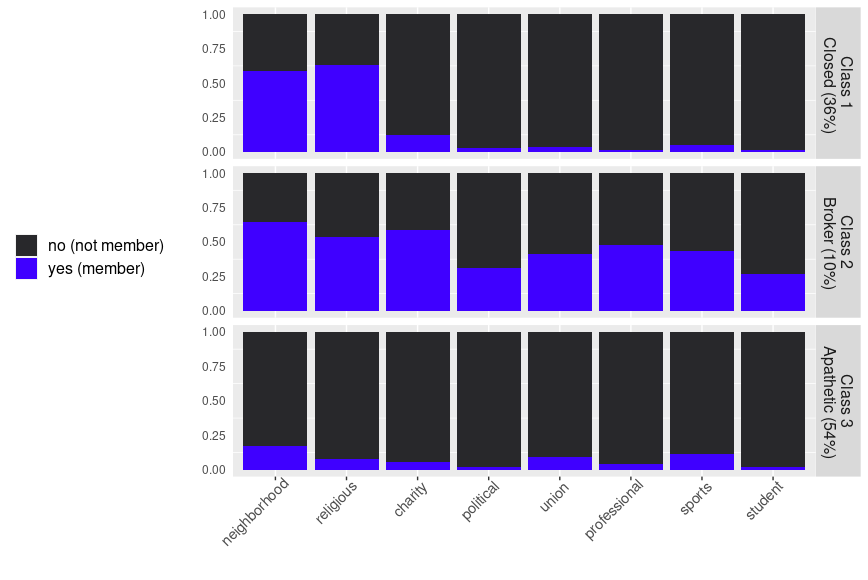
\includegraphics[width=15cm]{output/plot_latentclass.png}
    \caption{Estimates conditional response probabilities}
    \label{fig:galaxy}
\end{figure}


% latex table generated in R 4.1.2 by xtable 1.8-4 package
% Thu Jun  1 19:02:37 2023
\begin{table}[H]
\centering
\begin{threeparttable}
\caption{\label{demo-table} Multinomial regression}
\begin{tabular}{rrr}
  \hline
 & Class 2 (broker) & Class 3 (apathetic)\\ 
  \hline
Intercept & -1.66** & 1.56*** \\ 
  Mujer & -1.46*** & -1.32*** \\ 
  25-34 & 0.24 & -0.16 \\ 
  35-44 & 0.46 & -0.53 \\ 
  45-54 & 0.47 & -0.70 \\ 
  55-64 & -0.15 & -1.19** \\ 
  65- & -0.67 & -1.72*** \\ 
  Media & 0.82* & 0.49* \\ 
  Técnica & 1.40** & 1.00** \\ 
  Universitaria & 3.24*** & 1.57*** \\ 
   \hline
\multicolumn{3}{l}{\textsuperscript{***}$p<0.01$, 
  \textsuperscript{**}$p<0.05$, 
  \textsuperscript{*}$p<0.1$}
\end{tabular}
\begin{tablenotes}
    \item[1] Class 1 (closed) is reference category.
  \end{tablenotes}
\end{threeparttable}
\end{table}




\section{Discussion}

\section{Conclusion}

- The low level of membership in voluntary associations in Chile is notable.
- The associative behavior pattern that we call “broker” is the least numerous and least stable over time.
- It is remarkable that the pattrn “broker” accumulates the largest number of people who trust other strangers
- At the same time, it is the pattern that accumulates the most diversity.
- Finally, it is noteworthy that the pattern that least trusts others is the
closed one (which corresponds to our hypothesis) and that the difference, in favor of the “broker” class, is the strongest in relation to the others.

\newpage

\printbibliography

\newpage

\section{Supplementary analysis}

% Called in the psych package  fa2latex % Called in the psych package  fa % Called in the psych package    % Called in the psych package  Análisis Factorial Exploratorio Ola 1 
\begin{table}[htpb]\caption{Análisis Factorial Exploratorio Ola 1}
\begin{center}
\begin{scriptsize} 
\begin{tabular} {l r r r r r r }
 \multicolumn{ 6 }{l}{   } \cr 
 \hline Variable  &   PA1  &  PA3  &  PA2  &  $h^2$  &  $u^2$  &  com \cr 
  \hline 
c12\_01   &  0.12  &  0.04  &  \bf{0.66}  &  0.45  &  0.55  &  1.08& \cr 
 c12\_02   &  0.02  &  0.14  &  \bf{0.68}  &  0.48  &  0.52  &  1.08& \cr 
 c12\_03   &  \bf{0.55}  &  \bf{0.33}  &  0.30  &  0.50  &  0.50  &  2.26& \cr 
 c12\_04   &  \bf{0.66}  &  0.18  &  0.04  &  0.47  &  0.53  &  1.15& \cr 
 c12\_05   &  \bf{0.72}  &  0.29  &  0.05  &  0.61  &  0.39  &  1.33& \cr 
 c12\_06   &  \bf{0.45}  &  \bf{0.42}  &  \bf{0.39}  &  0.54  &  0.46  &  2.96& \cr 
 c12\_07   &  0.24  &  \bf{0.41}  &  0.04  &  0.23  &  0.77  &  1.65& \cr 
 c12\_08   &  0.26  &  \bf{0.96}  &  0.13  &  1.00  &  0.00  &  1.19& \cr 
 c12\_09   &  0.18  &  0.22  &  0.14  &  0.10  &  0.90  &  2.68& \cr 
\hline \cr & PA1  &  PA3  &  PA2  &  \cr 
 SS loadings & 1.65 &  1.56 &  1.18 &  \cr  
 \hline 
\end{tabular}
\end{scriptsize}
\end{center}
\label{default}
\end{table} 



\begin{table}[htpb]\caption{Análisis Factorial Exploratorio Ola 3}
\begin{center}
\begin{scriptsize} 
\begin{tabular} {l r r r r r r }
 \multicolumn{ 6 }{l}{   } \cr 
 \hline Variable  &   MR1  &  MR3  &  MR2  &  $h^2$  &  $u^2$  &  com \cr 
  \hline 
c12\_01   &  0.12  &  0.16  &  \bf{ 0.54}  &  0.33  &  0.67  &  1.27& \cr 
 c12\_02   &  0.08  &  0.05  &  \bf{ 0.74}  &  0.55  &  0.45  &  1.03& \cr 
 c12\_03   &  \bf{0.49}  &  \bf{0.49}  &  \bf{ 0.41}  &  0.65  &  0.35  &  2.92& \cr 
 c12\_04   &  0.24  &  \bf{0.62}  &   0.11  &  0.45  &  0.55  &  1.35& \cr 
 c12\_05   &  \bf{0.38}  &  \bf{0.75}  &   0.20  &  0.74  &  0.26  &  1.65& \cr 
 c12\_06   &  \bf{0.47}  &  \bf{0.32}  &  \bf{ 0.37}  &  0.46  &  0.54  &  2.72& \cr 
 c12\_07   &  \bf{0.57}  &  0.26  &  -0.01  &  0.39  &  0.61  &  1.41& \cr 
 c12\_08   &  \bf{0.78}  &  0.19  &   0.17  &  0.68  &  0.32  &  1.22& \cr 
 c12\_09   &  0.24  &  0.12  &   0.08  &  0.08  &  0.92  &  1.66& \cr 
\hline \cr & MR1  &  MR3  &  MR2  &  \cr 
 SS loadings & 1.68 &  1.43 &  1.23 &  \cr  
 \hline 
\end{tabular}
\end{scriptsize}
\end{center}
\label{default}
\end{table} 

\begin{table}[htpb]\caption{Análisis Factorial Exploratorio Ola 6}
\begin{center}
\begin{scriptsize} 
\begin{tabular} {l r r r r r r }
 \multicolumn{ 6 }{l}{   } \cr 
 \hline Variable  &   MR1  &  MR3  &  MR2  &  $h^2$  &  $u^2$  &  com \cr 
  \hline 
c12\_01   &   0.09  &   0.13  &  \bf{ 0.50}  &  0.28  &  0.72  &  1.22& \cr 
 c12\_02   &  -0.03  &  -0.07  &  \bf{ 0.75}  &  0.56  &  0.44  &  1.02& \cr 
 c12\_03   &  \bf{ 0.56}  &   0.22  &   0.26  &  0.43  &  0.57  &  1.75& \cr 
 c12\_04   &  \bf{ 0.58}  &   0.17  &  -0.02  &  0.36  &  0.64  &  1.18& \cr 
 c12\_05   &  \bf{ 0.74}  &   0.25  &   0.10  &  0.62  &  0.38  &  1.26& \cr 
 c12\_06   &  \bf{ 0.38}  &  \bf{ 0.41}  &  \bf{ 0.32}  &  0.41  &  0.59  &  2.88& \cr 
 c12\_07   &   0.28  &  \bf{ 0.49}  &   0.05  &  0.33  &  0.67  &  1.62& \cr 
 c12\_08   &   0.22  &  \bf{ 0.84}  &   0.09  &  0.76  &  0.24  &  1.16& \cr 
 c12\_09   &   0.14  &   0.14  &   0.22  &  0.09  &  0.91  &  2.44& \cr 
\hline \cr & MR1  &  MR3  &  MR2  &  \cr 
 SS loadings & 1.5 &  1.3 &  1.05 &  \cr  
 \hline 
\end{tabular}
\end{scriptsize}
\end{center}
\label{default}
\end{table} 


\end{document}
